\documentclass[11pt,
%twoside
]{article}


\usepackage[hyperfootnotes=false]{hyperref}                                    
\usepackage{amsmath,amsthm,amssymb}      
\usepackage{titlesec}                                                         
\usepackage{bm}        
\usepackage{cprotect}                                
%\usepackage{savetrees} 
\usepackage{bbold}
\usepackage{abstract}

\usepackage{tikz}
\usetikzlibrary{arrows}
                                          
\usepackage{graphicx}                                      
\graphicspath{{../figures/}, {../figures/growthrates/}, {../figures/correlations/}, {../python/Old_Hamiltonian/figures/}}

\usepackage[sorting=none, url=false, maxbibnames=5]{biblatex}
\bibliography{bib.bib}

% Formatting
\usepackage{indentfirst}
\usepackage{geometry}  
\geometry{inner=1.5in,outer=1in}
\geometry{margin=1in, lmargin=1.5in}
\usepackage{setspace}
\titleformat{\subsection}
{\normalfont\large\bfseries}{\thesubsection}{1em}{}
\renewcommand{\baselinestretch}{1.4}

\newcommand\blfootnote[1]{%
	\begingroup
	\renewcommand\thefootnote{}\footnote{#1}%
	\addtocounter{footnote}{-1}%
	\endgroup
}

\renewcommand{\bf}{\mathbf}
\renewcommand{\cal}{\mathcal}
\newcommand{\pd}[2]{\frac{\partial #1}{\partial #2}}
\newcommand{\pdn}[3]{\frac{\partial^{#3} #1}{\partial #2^{#3}}}
\newcommand{\pdop}[1]{\frac{\partial}{\partial #1}}
\newcommand{\nd}[2]{\frac{d #1}{d #2}}
\newcommand{\ndn}[3]{\frac{d^{#3} #1}{d #2^{#3}}}
\newcommand{\ndop}[1]{\frac{d}{d #1}}
\newcommand{\dt}{\frac{d}{dt}}
\newcommand{\grad}{\bm\nabla}
\newcommand{\cross}{\times}
\newcommand{\curl}{\grad\cross}
\newcommand{\imp}{\Longrightarrow\quad}
\newcommand{\abs}[1]{\left|#1\right|}
\newcommand{\half}{\frac{1}{2}}
\newcommand{\third}{\frac{1}{3}}
\renewcommand{\th}[1]{\frac{1}{#1}}
\renewcommand{\k}{4\pi\epsilon_0}
\newcommand{\eps}{\epsilon}
\newcommand{\intt}{\int_{t_1}^{t_2}}
\newcommand{\inti}{\int_{-\infty}^{+\infty}}
\newcommand{\ex}[1]{\left\langle #1 \right\rangle}
\newcommand{\oom}[1]{\times 10^{#1}}
\renewcommand{\d}{\delta}
\newcommand{\e}{\text{e}}
\renewcommand{\l}{\ell}
\newcommand{\om}{\omega}
\newcommand{\h}{\hbar}
\newcommand{\ket}[1]{\left|#1\right\rangle}
\newcommand{\bra}[1]{\left\langle#1\right|}
\newcommand{\braket}[2]{\left\langle#1\middle|#2\right\rangle}
\newcommand{\brakett}[3]{\left\langle#1\middle|#2\middle|#3\right\rangle}
\newcommand{\nn}{\nonumber\\}

\DeclareMathOperator{\Tr}{Tr}
\let\Re\relax
\DeclareMathOperator{\Re}{Re}

\begin{document}
	
\pagenumbering{Roman}
\begin{titlepage}
{\setstretch{1.5}
\vspace*{.2in}
\begin{center}
	\huge{\textbf{Operator and Entanglement Dynamics \\
			        in Asymmetric Quantum Systems}}
\end{center}
\vspace{.6in}
\sc
\begin{center}
	\LARGE{Charles Nicholas Stahl}
\end{center}
\vspace{.6in}
\begin{center}
\today
\end{center}
\vspace{.6in}
\begin{center}
	{\Large Advised by Professor David Huse} \\
	Second Reader: Professor Shivaji Sondhi
\end{center}
\vspace{.6in}
\begin{center}
	Submitted in partial fulfillment \\
	of the Requirements for the \\
	Degree of Bachelor of Arts
\end{center}
}
\newpage

\begin{abstract}
	Thermalization is an important aspect in quantum physics from condensed matter to black holes. It allows initially local information to be spread and hidden throughout a system. This spreading happens at a finite speed, and can be quantified using the butterfly velocity $v_B$ or the entanglement velocity $v_E$. These speeds are well-studied, and are independent of each other up to the constraint $v_B>v_E$. Although it is possible to have a direction-dependent $v_B$, little work has been done to study systems like this. In this thesis we study two systems on spin chains with asymmetric butterfly velocities, which we call $v_{B\pm}$. In the first, a system with a time-independent Hamiltonian, we study $v_B$ through operator spreading. We show that the system is slightly asymmetric, with $v_{B+}>v_{B-}$. The second system is a quantum circuit with random unitary dynamics. Using entanglement dynamics to measure the butterfly velocity, we show that these systems can have $v_{B+}/v_{B-}$ arbitrarily large.\blfootnote{I pledge my honor that this paper represents my own work in accordance with University regulations. \vspace*{1in}}
\end{abstract}

\newpage

\section*{Acknowledgments}

Thank you, Professor Huse, for making this project possible. Your availability and willingness to meet made my senior thesis process tractable, interesting, and so much fun. From patiently explaining the necessary background material, even when I had just asked the same questions last week, to suggesting useful new directions to explore and helping me interpret the results, you made my foray into quantum information dynamics painless and engaging. 

Professor Sondhi, thank you for all you have done to expand my physics knowledge, from advising my summer and future plans, to agreeing to advise an extra math class this semester, to being my second reader, I will always appreciate your helpfulness throughout my last two years in the department. 

Thank you Witherspoon 517+, for simultaneously backing me up and pushing me forward  since freshman year. I can't imagine being placed in a better freshman hall. I can never catch a break with you guys, but that constant needling got me here, so I can't really complain.

To the seniors and assorted juniors who have made the physics department a comfortable place for me, thank you for getting me through four years of classes and independent work without losing my mind. I'm lucky to have been in such a cohesive department with so much positive encouragement between students.

Mom, Dad, Maria, thank you for being the smartest, funnest, and most interesting family I've ever had. You have instilled in me a love for science, a love for wit, and a love for knowledge that have made me who I am today. Mom and Dad, I know I would never be here without you. And Maria, I am so lucky to have been able to spend so much time with you over the past two years on campus. You're an inspiration.

And as always, thank you Haley for five wonderful years of love and support. Knowing that, no matter how hard a day has been, you will be ready to listen and understand on the phone gives me a fabulous feeling of peace. I can't wait to see where our next five years of adventures take us. I love you to the moon and back!

\newpage

\tableofcontents
\end{titlepage}
\cleardoublepage
\pagenumbering{arabic}
\input{introduction}
\clearpage
\section{Operator Spreading in Time-Independent Hamiltonian Systems} \label{sec:opsp}

Just do all intro here, and then decide later what to put into the circuit section

Thermalization 
  vs localization 
  happens by spreading information
  mention that this is how information loss happens

Discuss information movement in Time-Independent Hamiltonian systems
  Find a source for this
  Ideally introduce OTOC and Pauli end weight here
  Also entanglement possibly
  What is the relationship between entropy and OTOC?
  Argument about extremal slope
    From Nahum: stairs to separate $v_B$ and $v_E$ - It is possible to make $v_E << v_B$ in quantum circuit architectures [CITE], which will be discussed in section~\ref{sec:circuits}
    

For now use Jonay paper, but hopefully find another. Could use Keyserlingk but it would be nice to save that for the discussion of random unitary dynamics.

Although most sources consider symmetric dynamics [CITE] this is not a requirement. Find the Nahum paper that discusses asymmetric systems.

\hrule

All systems considered in this thesis will exist on spin chains, one-dimensional collection of quantum degrees of freedom. Initially we consider systems with $q=2$ degrees of freedom at each site, such as a chain of spin-$\half$ particles. Later, we will consider sites with more degrees of freedom. 

Under a time-independent Hamiltonian $H$, states of the system evolve in the Schr\"odinger picture as 
\begin{align}
\ket{\psi(t)} = U(t)\ket{\psi(0)},\quad U(t) = \e^{-iHt}. \label{eqn:shro}
\end{align}
This evolution can be generalized to a time-dependent Hamiltonian by evolving with the time-ordered unitary operator
\begin{align}
U(t,t_0) = \text{T}\e^{-i\int_{t_0}^td\tau H(\tau)}.\nonumber
\end{align}
As we will consider time-independent Hamiltonians, we only need time evolution operators of the form of equation~\ref{eqn:shro}.

Instead of evolving states, it is possible to evolve operators under the Heisenberg picture. In order to preserve the time dependence of expectation values, the operators must evolve as 
\begin{align}
A(t) = U^\dag(t)\,A(0)\,U(t) = \e^{iHt}A(0)\,\e^{-iHt}.\label{eqn:heis}
\end{align}

One remark worth making about time evolution in different pictures is that operators aren't the only the only important Hermitian matrix in the system. The density matrix $\rho$ describes the state of the system, and in pure states is $\rho = \ket{\psi}\bra{\psi}$. Density matrices are more general than kets, though, because they can represent mixed states. In the Schr\"odinger picture $\rho$ evolves the way its construction would imply
\begin{align}
\rho(t) = \e^{-iHt}\rho(0)\e^{iHt}
\end{align}
while it does not evolve in the Heisenberg picture. This is the opposite of observables, so when discussing the evolution of matrices it is necessary to specify whether they are observables or density matrices.

\subsection{Pauli Strings and Pauli Weight} \label{sub:pauli}

This subsection is based on~\cite{Keyserlingk}. When discussing operator spreading it is convenient to decompose operators that may act on very high dimensional Hilbert spaces into the Pauli basis. The basis operators are tensor products of Pauli matrices. Eventually we will decompose operators that are initially local, but any operator can be decomposed in this manner.

For single sites with Hilbert spaces of complex dimension $q$, the space of Hermitian operators is $q^2$-dimensional.\footnote{Check this. Something is off.} For $q=2$ the basis operators are $X, Y, Z, I$. In general, the operators will be of the form 
\begin{align}
\sigma^\mu = X^{\mu_1}Z^{\mu_2},
\end{align}
where $\mu_1, \mu_2\in\{0,1,\dots,q-1\}$\footnote{How to get Y?}. Under the matrix norm $||M|| = \text{tr}(M^\dag M)/q$, this basis is orthonormal:
\begin{align}
\th{q}\text{tr}(\sigma^{\mu\dag}\sigma^\nu) &= \th{q}\text{tr}(Z^{\mu_2\dag}
	X^{\mu_1\dag}X^{\nu_1}Z^{\nu_2})\nn
&= \delta_{\mu\nu}.\label{eqn:orthonorm}
\end{align}

A general operator $A$ evolves into
\begin{align}
A(t) = U^\dag(t)A\,U(t) = \sum_\nu c_\nu(t)\sigma^\nu.\label{eqn:decomp}
\end{align}
Due to the orthonormality, the coefficients are 
\begin{align}
c_\nu(t) = \th{q}\text{tr}(\sigma^{\nu\dag}A(t))
\end{align}
and obey $\sum_\nu \abs{c_\nu}^2 = 1$.

With $c_\nu(t)$ in hand, we can define the Pauli weight $W(i,t)$ as how much of the weight of the operator is on Pauli strings that end on site $i$:
\begin{align}
W(i,t) = \sum_\nu\abs{c_\nu(t)}^2\delta(\text{end}(\nu)=i).
	\label{eqn:endweight}
\end{align}
The delta function constrains the sum to be only over $\nu$ such that $\sigma^\nu$ has a non-identity at site $i$ and identities at all sites right of $i$. Reference~\cite{Keyserlingk} refers to this quantity as $\rho$ to emphasize its hydrodynamic evolution. It is possible to define an analogous quantity with the sum over strings that begin on site $i$- those which have non-identities on all sites left of $i$. In that case the quantity in equation~\ref{eqn:endweight} can be called $W_R(i,t)$ while the weight of sites that start on $i$ is $W_L(i,t)$.

As an example, write
\begin{align}
A = X_1\otimes Y_2\otimes Y_3\otimes I_4 + I_1\otimes I_2\otimes Z_3\otimes Z_4,
	\nonumber
\end{align}
where the subscript designates the site on which each operator acts. This can be shortened to
\begin{align}
A = XYYI + IIZZ\label{eqn:inioper}.
\end{align}

This decomposition is particularly useful when the initial operator is local. This means that all strings in the Pauli decomposition contain non-identiy operators at a single site. Then the end weights describe how far the operator has spread throughout the system due to the unitary dynamics. \emph{Mention thermalization} \emph{figure from Jonay}

The Pauli weight is closely related to the Out-of-Time-Ordered Correlator (OTOC). Consider an initial operator, say, $A(0)=Z_1=ZII\dots$. This will commute with operators that are local at other sites and later times, $B(x,t)$. However, in general the time-evolved $A(t)$ will include Pauli strings that have non-identity operators at all sites. This can be seen through the Baker-Campbell-Hausdorff expansion~\cite{Roberts2016} of the time evolution
\begin{align}
A(t) &= \e^{iHt}A(0)\e^{-iHt} \nn
&= \sum_k\frac{(it)^k}{k!}[H,[H,\dots[H,A(0)]\dots]]
\end{align}

Find Pauli weight. Discuss name, way to calculate. Relate to OTOC

Find weight at site.

\subsection{Entanglement Entropy} \label{sub:intro}

Quantum entanglement describes aspects of branches of physics from high energy and quantum information theory to experimental studies of cold atomic gases. Although entanglement is so widely studied, its dynamics are less well understood. The dynamics of the entanglement entropy are closely related to the speed at which information travels or spreads. 
%One way to study this topic is to consider entanglement dynamics of spin chains. 

Entanglement entropy provides one way to quantify the entanglement and is defined as follows. For a system $AB$ divisible into subsystems $A$ and $B$, the reduced density matrices $\rho_A$ and $\rho_B$ are the full density matrix $\rho_{AB}$ traced over subsystem $B$ and $A$, respectively. If the full system is in a pure state, the $n$th Renyi entropy of density matrix $\rho$ is 
\begin{align}
S_n = \th{1-n}\log\left(\Tr\rho^n\right). \label{eqn:renyi}
\end{align}
In the limit $n\to1$ this becomes the von Neumann entropy
\begin{align}
S_{vN} = -\Tr\rho\log\rho,
\end{align}
the analogue of the classical Shannon entropy. These entropies are maximized by maximally mixed states, with entropy $N\log q$ for $N$-site systems with $q$-dimensional Hilbert spaces at each site.

Introduce entropy bounds here.

References~\cite{Keyserlingk, Jonay} discuss the speed of entanglement in brickwork models using related concepts called out of time order commutator (OTOC) and operator density. Reference~\cite{Zhou2017} quantifies the scrambling using the operator entanglement entropy opEE of the time evolution operator.

\subsubsection{Entropy Constraints} \label{subsub:constraints}

The following description is largely taken from~\cite{Nahum2017}. Consider a spin chain of N sites with dimension $q$. $q=2$ corresponds to spin-$\half$ particles, $q=3$ corresponds to spin-1 particles, etc. Sites are labeled by $i=1,\dots N$, while the bonds between sites are labeled by $x = 1,\dots N-1$. After cutting the system at bond $x$, define the entropy across this cut as the bipartite entanglement entropy of all sites to the right of $x$. If the whole chain is in a pure state, this is equal to the bipartite entanglement entropy of all sites to the left of $x$.

The von Neumann entropy at cut $x$ is
\begin{align}
S(x) = \-\Tr\rho_x\log\rho_x, \label{eqn:vonneu}
\end{align}
where $\rho_x$ is the density matrix of the system with all sites left of $x$ traced out, and for convenience logarithms are taken base $q$. Classically, for an arbitrary system decomposable into subsystems $A$ and $B$, the entropies satisfy $\max(S(A), S(B)) \leq S(AB)\leq S(A) + S(B)$. In quantum mechanics, this is replaced by the subadditivity of the von Neumann entropy 
\begin{align}
\left|S(A)-S(B)\right| \leq S(AB)\leq S(A) + S(B). \label{eqn:subadd}
\end{align}
If we take subsystem $A$ to be the single site between cuts $x$ and $x+1$ and subsystem $B$ to be all sites right of $x+1$, this becomes
\begin{align}
\left|S_1 - S(x+1)\right| \leq S(x) \leq S_1 + S(x+1),
\end{align}
where $S_1$ denotes the entropy of the single site between cuts $x$ and $x+1$. After some rearranging this can be written $\left|S(x+1) - S(x)\right| \leq S_1$. However, since the single site is $q$ dimensional, $S_1 \leq \log q = 1$, explaining the use of $q$ for the base. The preceding arguments taken together give the constraint
\begin{align}
\left|S(x+1) - S(x)\right| \leq 1. \label{eqn:offbyone}
\end{align}

\clearpage
\section{Dynamics in an Asymmetric Hamiltonian} \label{sec:asymham}

\subsection{3-Site Hamiltonian} \emph{} \label{sub:hamiltonian}

Instead of a Floquet or quantum circuit system, we can consider one with a time-independent Hamiltonian, for a finite number of dimensions at each site. We can choose a Hamiltonian based on how uneven its dynamics are. For example, the three-site swap $S_{123}$ is a unitary operator such that 
\begin{align}
S_{123}\psi_1\psi_2\psi_3 =\psi_2\psi_3\psi_1, \label{eqn:condition}
\end{align}
where the position of the wavefunction denotes the site on which it sits. 

One way to build the three site swap gate is in a Floquet system, out of two site swap gates $S_{123} = S_{23}S_{12}$. However it is also possible to build it out of a time-independent Hamiltonian, so that $U(1) = \e^{-iH_3} = S_{123}$. This is possible by either taking the matrix-log of $S_{123}$ or by considering the eigenstates and corresponding eigenvalues. 

For a spin-$\half$ system, there will be 8 states, which can be decomposed into a spin-$\frac{3}{2}$ subspace with 4 states and 2 spin-$\half$ subspaces with 2 states each. The eigenstates will be states in which individual particle states differ only by phases. There are four states that should not change in time and therefore have 0 energy. Before normalization these are
\begin{align}
\ket{000},\quad \ket{100}+\ket{010}+\ket{001},\nn
\ket{111},\quad \ket{011}+\ket{101}+\ket{110}.\label{eqn:zero}
\end{align}
Of the four other states, two should have positive energy and two should have negative energy. Since $U(3)=1$, their energies should be $E_\pm = \pm\frac{2\pi}{3}$ so they pick up a phase $\phi_\pm =\e^{-iE_\pm} = \e^{\mp i\frac{2\pi}{3}}$. Using condition~\ref{eqn:condition}, we can show that the positive energy states are
\begin{align}
&\ket{100} + \phi_-\ket{010} + \phi_+\ket{001},\nn
&\ket{011} + \phi_-\ket{101} + \phi_+\ket{110},\label{eqn:plus}
\end{align}
while the negative energy states are 
\begin{align}
&\ket{100} + \phi_+\ket{010} + \phi_-\ket{001},\nn
&\ket{011} + \phi_+\ket{101} + \phi_-\ket{110}.\label{eqn:minus}
\end{align}

In matrix notation, with basis states $\ket{000},\,\ket{001},\,\ket{010},$ etc, the hamiltonian is 
\begin{align}
H_3 = T\; \text{diag}(0,0,0,0,E_+,E_+,E_-,E_-)\; T^\dag,
\end{align}
where $T$ is the transformation matrix suggested by~\ref{eqn:zero}, \ref{eqn:plus}, and~\ref{eqn:minus},
\begin{align}
T = \th{\sqrt{3}}\begin{bmatrix}
\sqrt{3} & 0 & 0 & 0        & 0      & 0      & 0      & 0      \\
0        & 1 & 0 & 0        & \phi_+ & 0      & \phi_- & 0      \\
0        & 1 & 0 & 0        & \phi_- & 0      & \phi_+ & 0      \\
0        & 0 & 1 & 0        & 0      & 1      & 0      & 1      \\
0        & 1 & 0 & 0        & 1      & 0      & 1      & 0      \\
0        & 0 & 1 & 0        & 0      & \phi_- & 0      & \phi_+ \\
0        & 0 & 1 & 0        & 0      & \phi_+ & 0      & \phi_- \\
0        & 0 & 0 & \sqrt{3} & 0      & 0      & 0      & 0
\end{bmatrix}
\end{align}
Altogether
\begin{align}
H_3 = \frac{2\pi i}{\sqrt{3}}\begin{bmatrix}
0 & 0  & 0  & 0  & 0  & 0  & 0  & 0 \\
0 & 0  & 1  & 0  & -1 & 0  & 0  & 0 \\
0 & -1 & 0  & 0  & 1  & 0  & 0  & 0 \\
0 & 0  & 0  & 0  & 0  & -1 & 1  & 0 \\
0 & 1  & -1 & 0  & 0  & 0  & 0  & 0 \\
0 & 0  & 0  & 1  & 0  & 0  & -1 & 0 \\
0 & 0  & 0  & -1 & 0  & 1  & 0  & 0 \\
0 & 0  & 0  & 0  & 0  & 0  & 0  & 0 \\
\end{bmatrix}
\end{align}

This hamiltonian should be symmetric under a simultaneous rotation of all three spins, so that it can be written as $H_3(\bm{\sigma}_1,\,\bm{\sigma}_2 ,\,\bm{\sigma}_3)$. It should be antisymmetric under the interchange of any two spins (equivalent to reversing the direction of propagation). The only function of three vectors that has this property is the triple product $H_3= \bm{\sigma}_1\cdot\left(\bm{\sigma}_2 \times\bm{\sigma}_3\right)$.

%Note that this is equivalent to
%\begin{align}
%H &= \bm{\sigma}_1\cdot\left(\bm{\sigma}_2 \times\bm{\sigma}_3\right) \nn
% &= \sigma_{1,1}\otimes\sigma_{2,2}\otimes{\sigma}_{3,3} - {\sigma}_{1,1}
%	\otimes\sigma_{2,3}\otimes\sigma_{3,2} + \sigma_{1,2}\otimes{\sigma}_{2,3} \otimes {\sigma}_{3,1}-\cdots
%\end{align}

Exponentiating the hamiltonian gives the time evolution operator for one time step
\begin{align}
U(1) = \e^{-iH_3} = \begin{bmatrix}
1 & 0 & 0 & 0 & 0 & 0 & 0 & 0 \\
0 & 0 & 1 & 0 & 0 & 0 & 0 & 0 \\
0 & 0 & 0 & 0 & 1 & 0 & 0 & 0 \\
0 & 0 & 0 & 0 & 0 & 0 & 1 & 0 \\
0 & 1 & 0 & 0 & 0 & 0 & 0 & 0 \\
0 & 0 & 0 & 1 & 0 & 0 & 0 & 0 \\
0 & 0 & 0 & 0 & 0 & 1 & 0 & 0 \\
0 & 0 & 0 & 0 & 0 & 0 & 0 & 1
\end{bmatrix}
\end{align}
This has the properties of of condition~\ref{eqn:condition}. Furthermore, application three times gives $U(3) = 1$. The hamiltonian commutes with the total spin-Z operator $S_Z = \text{diag}(\frac{3}{2}, \frac{1}{2}, \frac{1}{2}, -\frac{1}{2}, \frac{1}{2}, -\frac{1}{2}, -\frac{1}{2}, -\frac{3}{2})$ so total spin-Z is conserved. It also commutes with the other components of spin and therefore also total spin $S^2$.

If the system starts in a computational basis state, for example $\ket{100}$, the coefficients for the other states with equal total spin-Z will both change from 0 before the states becomes $\ket{010}$ at time 1, as in figure~\ref{fig:timeevol}.
\begin{figure}
	\centering
	\includegraphics[width=.5\textwidth]{timeevol}
	\caption{Evolution of coefficients if the system starts in state $\ket{100}$.}
	\label{fig:timeevol}
\end{figure}

\subsection{Multi-Site Hamiltonian} \emph{}\label{sub:multistate}

\subsubsection{Construction} \label{subsub:construction} \emph{}

There are multiple ways to extend this hamiltonian to a chain of $L= 2n+1$ spins. Like building $S_{123}$ out of two-site swaps we can treat the larger system as a Floquet system, successively applying $H_3$ to each triplet of spins. We can define a similar hamiltonian by putting the 3-site hamiltonian simultaneously on sites 1-3, sites 3-5, etc. For $n=2$, this is
\begin{align}
H_5 = H_3\otimes\mathbb{I}_2 + \mathbb{I}_2\otimes H_3.
\end{align} 
This hamiltonian still preserves each component of total spin. 

Starting in $\ket{00001}$, the coefficients follow the pattern of figure~\ref{fig:timeevol5}. At first the evolution is similar to the $n=1$ case, with $\ket{10000}$ and then $\ket{01000}$ reaching near maximal. The coefficient of $\ket{00001}$ is 
\begin{align}
\frac{1}{10} \left(3 \cos \left(\frac{2}{3} \sqrt{\frac{5}{3}} \pi  t\right)+5 \cos \left(\frac{2 \pi  t}{3 \sqrt{3}}\right)+2\right)
\end{align} 
which is shown in figure~\ref{fig:onecoef}. Although it appears to be quasi-periodic, it cannot ever reach 1 for $t\ne 0$ or be truly periodic because its time coefficients are not rationally related.

\begin{figure}
	\centering
	\includegraphics[width=.5\textwidth]{timeevol5}
	\caption{Evolution of coefficients if the system starts in state $\ket{00001}$.}
	\label{fig:timeevol5}
\end{figure}

\begin{figure}
	\centering
	\includegraphics[width=.5\textwidth]{onecoef}
	\caption{Coefficient for $\ket{00001}$ when that is the starting state.}
	\label{fig:onecoef}
\end{figure}

%The coefficient for $\ket{00100}$ does not fit the pattern. It does not reach maximum at the right time and it does have a periodic structure. Furthermore, when the starting state is $\ket{00010}$ the problematic state is still $\ket{00100}$, probably because of the chaining mechanism. When the starting state is $\ket{00100}$ the coefficients for $\ket{10000}$ and $\ket{00001}$ always vanish. The next chaining method to try will be to have $2n$ spins, and to have the first spin complete the last trio.

\subsubsection{Pauli String Weight} \label{subsub:operator_dynamics} \emph{} 

We can study the operator dynamics of this system by extending to large $L$ and evolving operators that are identities on all sites except one end. Since the hamiltonian is SO(3) symmetric, it does not matter if the perturbation is $X$, $Y$, or $Z$. For convenience, we will use $Z$. We can then study the weight of strings that end at each site $i$, $W(t; i)$.

For the forward-propagating wave, with $A(t=0) = Z_0 = Z\otimes \mathbb{I} \otimes \mathbb{I} \cdots$, the weight starts on site 0 and peaks at even sites. The successive peaks fall off in size but dominate the Pauli strings until the last site takes over (figure~\ref{fig:L11end3n20front}). This is possibly because 

For the backward-propagating waves $(A(t=0)=Z_{L-1})$, the initial decaying signal is more difficult to make out but still present. It is dominated by a large weight of sites that start on site 9 around $t=1$. By $t = 3$ the first site has started to dominate the Pauli weights.

\begin{figure}
	\centering
	\includegraphics[width=.7\textwidth]{L11end3n20front}
	\caption{Weight of operators that end on site $i$.}
	\label{fig:L11end3n20front}
\end{figure}
\begin{figure}
	\centering
	\includegraphics[width=.7\textwidth]{L11end3n20back}
	\caption{Weight of operators that begin on site $i$.}
	\label{fig:L11end3n20back}
\end{figure}

The initial behavior also matches the $L=9$ case. For forward propagation the initial behavior is $W(t;i) = a\e^{bt}$ with $a,b$ given by\dots Figure~\ref{fig:L11end1n60fore} shows this behavior, while figure~\ref{fig:L11end1n60back} shows the analogous behavior for the backward propagating wave. 

\begin{figure}
	\centering
	\includegraphics[width=.7\textwidth]{L11end1n60fore}
	\caption{Early-time leading edge weights for forward propagating wave.}
	\label{fig:L11end1n60fore}
\end{figure}
\begin{figure}
	\centering
	\includegraphics[width=.7\textwidth]{L11end1n60back}
	\caption{Early-time leading edge weights for backward propagating wave.}
	\label{fig:L11end1n60back}
\end{figure}

Here the relevant numbers are\dots
Again, the exponents for even and odd sites increase by one within each group. Pairs of sites separated by 3 are also divergent in the forward case while convergent in the backward case.
\clearpage
\section{Entanglement and Operator Spreading in Quantum Circuits} \label{sec:circuits}

\subsection{Circuit Architectures} \label{sub:arch}

Instead of evolving the spin chains with Hamiltonians, we can focus on quantum circuits. Like the earlier systems, circuits consist of chains of Hilbert spaces. Instead of evolving under a time-independent hamiltonian, they evolve with unitary operators, called gates, at discrete times. Simple circuits only contain 2-site gates which act on the product of Hilbert spaces at adjacent sites. 

We could study the dynamics of a single circuit, in analogy with the single hamiltonian studied in the previous section. However, it is also instructive to look at ensembles of circuits, with some type of randomness. This section presents two sources of randomness, the choice of gates and their locations in the circuit.

%References~\cite{Keyserlingk} and~\cite{Nahum2017} both discuss circuits of this type. Both discuss random circuits, although with different sources of randomness. 
One source is the unitary operator chosen at each site at each time. Different gates result in different architectures. 
If the Hilbert space at each site is $q$ dimensional, the space of 2-site unitary matrices is $q^2\times q^2$ dimensional. To find representative behavior, each circuit is made by drawing gates from some distribution. The circuits can then be averaged over these choices. 

Another source of randomness is the placement of the gates. The ``brickwork" model~\cite{Keyserlingk} uses a deterministic architecture, in which at odd times there is a gate to the right of every odd site, while for even times there is a gate to the right of every even site. The ``random" architecture~\cite{Nahum2017} chooses a random site for a single gate at each time step $t = n/\Gamma$, where $\Gamma$ is the gate rate and $n$ is an integer. The placement is then averaged over. The random architecture is equivalent to placing gates at each site in continuous time with Poisson-distributed time steps~\cite{Nahum2017}.

We will first discuss the brickwork circuit, shown in figure~\ref{fig:brickcircuit}.\footnotetext{Redo this figure without course graining, or with new labels.}
\begin{figure}
	\centering
	\input{brickcircuit}
	\caption{\textbf{Brickwork circuit architecture}. The red circles represent the initial states of the system, while the blue rectangles are unitary gates that evolve the system in time. The Hilbert space at each site is $q$-dimensional, meaning the gates are $q^2\times q^2$ matrices, chosen from the Haar distribution. Taken from~\cite{Keyserlingk}.}
	\label{fig:brickcircuit}
\end{figure}
In this model, each gate is chosen from the Haar distribution, which is invariant to rotations in the space of 2-site operators. Since these act on a $q^2$-dimensional Hilbert space, there are $q^4$ independent operators, including one trivial operator (the identity). 

We want to know how the Pauli end-weight $W(t,i)$ evolves in time in these circuits. Recall that, given an observable $\cal{O}(t)$ evolving in time, this measure how far $\cal{O}$ has spread. Consider the components of the operator that are identities after site $i$, which will have weight $W(t, i)$ by definition. Of the $q^2$ operators that can act on sites $i$ and $i+1$, $q^2$ will be trivial on the second site. Since these will not advance the Pauli end-weight, they do not contribute to operator spreading. 

\emph{Show an explicit example of this for $q=2$}

If some component of the observable ends on site $i+1$, the unitary can move the end back, if it evolves the observable at $i+1$ to the identity. Again, $q^2$ of the 2-site operators contain this specific unitary acting on the second site, so that the probability of moving weight from site $i+1$ to $i$ is the same as not moving the weight from $i$ to $i+1$.

Since the identity will never contribute to operator spreading, we can exclude it from our set of gates. Then, $q^4-q^2$ operators move the Pauli weight. The probability that a random gate advances $W(t,i)$ is $p = \frac{q^2}{q^2+1}$, so that $1-p = \frac{1}{q^2+1}$. After averaging over the possible circuits, this leads to the dynamics of $W(t,i)$, from~\cite{Keyserlingk}
\begin{align}
W(t+1, i) = (1-p)\left(W(t, i) + W(t, i+1)\right)\nn
W(t+1, i+1), = p\left(W(t, i) + W(t, i+1)\right).
\end{align}

[\emph{How much more detail should I go into before this just becomes a synopsis of their paper?}]

The butterfly speed is
\begin{align}
v_B= \frac{q^2-1}{q^2+1}. \label{eqn:keysvb}
\end{align}
The entanglement speed is 
\begin{align}
v_E = \frac{\log\frac{q+q^{-1}}{2}}{\log q} = \frac{\log\left(1-v_B^2
	\right)}{\log\left(\frac{1-v_b}{1+v_B}\right)}.\label{eqn:keysve}
\end{align}
These speeds describe operator spreading represented in figure~\ref{fig:onesite_spreading}.
\begin{figure}
	\centering
	\includegraphics[width=.5\linewidth]{onesite_spreading}
	\caption{\textbf{Operator spreading in a brickwork circuit}. $\bar{\rho_R}$ is what is here called $W(t,i)$. From~\cite{Keyserlingk}.}
	\label{fig:onesite_spreading}
\end{figure}
An initially local operator spreads with velocity $v_B$, and diffuses at a rate related to $v_E$. 

\subsection{Deterministic Limit}  \label{sub:determ}

Take the large $q$ limit of equations~\ref{eqn:keysvb} and~\ref{eqn:keysve}
\begin{align}
v_B &\simeq 1-\frac{2}{q^2},\nn
v_E &\simeq 1-\frac{\log 2}{\log q}.
\end{align}
Since both speeds approach the light cone velocity (defined to be 1), an initial perturbation does not spread in time, and travels at the light cone velocity. In figure~\ref{fig:onesite_spreading}, this would be represented by $\bar{R}$ and $\bar{L}$ becoming step functions and $W(t,i)$ becoming a delta function.

\emph{What are the two velocities in the random circuit architecture now?}

\emph{Make the connection to bipartite entanglement entropy for a state}

We know then that, except for fine-tuned operators that are measure zero on the Haar distribution, the random two-site gate will maximize bipartite entanglement entropy. From equation~\ref{eqn:offbyone} the maximum entanglement possible across cut $x$ is 
\begin{align}
S(x) \le \min\left\lbrace S(x-1), S(x+1)\right\rbrace + 1. \nonumber
\end{align}
Furthermore, a gate acting across cut $x$ does not affect $S(x-1)$ or $S(x+1)$.

Taken together, these facts mean that after a gate across cut $x$, the new entanglement entropy is~\cite{Buyskikh2016}~\emph{Make sure this is actually in this source}
\begin{align}
S(x, t+1) = \min\left\lbrace S(x-1, t), S(x+1, t)\right\rbrace + 1.
	\label{eqn:update}
\end{align}
Then if at any point $S(x)$ becomes integer valued, it remains so for the rest of the evolution. There are a few pictures that make this integer-valued evolution more intuitive.

\subsubsection{Surface Growth Picture}  \label{subsub:surfgrowth}

One model for the entropy growth described above is the Tetris-like surface growth picture. Here, the entropy is represented by a piecewise-constant function with the height given by the entropy across each cut, as in figure~\ref{fig:tetris}, taken from \cite{Nahum2017}. 
\begin{figure}
	\centering
	\includegraphics[width=.5\textwidth]{tetris.pdf}
	\caption{\textbf{Tetris-like model for large-$q$ chain.} The gate at cut $x$ adds enough entropy so that $S(x)$ is one greater than either of its neighbors. Figure from~\cite{Nahum2017}.}
	\label{fig:tetris}
\end{figure}
In general, it is possible for the entropy across two adjacent cuts to be equal. However, figure~\ref{fig:applyingUnitary}, also from~\cite{Nahum2017}, shows that flat sections can be destroyed but not created. 
\begin{figure}
	\centering
	\includegraphics[width=.5\textwidth]{applyingUnitary.pdf}
	\caption{\textbf{Several possibilities for local changes} in the large $q$ model. If three adjacent cuts all have equal entropy, the two flat sections annihilate each other. There is no way to generate flat sections.}
	\label{fig:applyingUnitary}
\end{figure}

It makes sense then to only consider states that have no flat sections, so that $S(x) = S(x-1)\pm1$ for all $x$. In this case, instead of a picture like figure~\ref{fig:tetris} it is possible to represent the entropy at each bond as a point, with a diagonal slope connecting bonds. The slope between cuts (at a site) will always be $\pm1$. Instead of $2\times1$ or $1\times1$ rectangles, the gates are then squares coming down point-first, as in figure~\ref{fig:diaggate}. 
\begin{figure}
	\centering
	\input{diaggate}
	\caption{\textbf{Another picture of the configuration in figure~\ref{fig:tetris}}. Here the cut positions are top or bottom vertices of the squares. On the left, the gate at time $t$ results in entropy growth at $x$ because at time $t-1$, $S(x-1) > S(x) < S(x+1)$. On the right the gate has no effect. Although $S(x) < S(x+1)$, the case $S(x) < S(x-1)$ is not satisfied. }
	\label{fig:diaggate}
\end{figure}
If the gate falls on a local minimum, it lifts the entropy at that bond. If the gate falls on a local maximum or a non-extremum it has no effect.

\subsubsection{Minimal Cut Picture} \label{subsub:mincut}

Using the fact that a productive gate raises the entropy at a cut by 2, we can use another picture of the dynamics based on figure~\ref{fig:brickcircuit}. Assume the initial state is a product state so the entropy at each cut is initially 0 and evolve with a brickwork circuit. Then after one of the first gates (for example between $i=3$ and $i=4$) the entropy at that cut will become 1. After any of the subsequent gates the entropy at the affected cut increases by 2.

The minimal cut picture~\cite{Nahum2017}\footnote{This might not be the original source} reproduces this behavior by considering cuts through the circuit, as in figure~\ref{fig:mincut}.
\begin{figure}
	\centering
	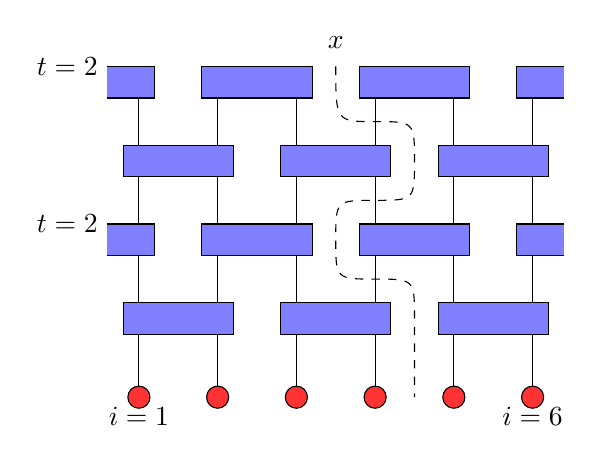
\begin{tikzpicture}[scale = 1]
\draw (0,0) node[below]{$i=1$} -- (0,4);
\filldraw[color=black, fill=red!80] (0,0) circle (4pt) node[anchor=west] { };
\draw (1,0) -- (1,4);
\filldraw[color=black, fill=red!80] (1,0) circle (4pt) node[anchor=west] { };
\draw (2,0) -- (2,4);
\filldraw[color=black, fill=red!80] (2,0) circle (4pt) node[anchor=west] { };
\draw (3,0) -- (3,4);
\filldraw[color=black, fill=red!80] (3,0) circle (4pt) node[anchor=west] { };
\draw (4,0) -- (4,4);
\filldraw[color=black, fill=red!80] (4,0) circle (4pt) node[anchor=west] { };
\draw (5,0) node[below]{$i=6$} -- (5,4);
\filldraw[color=black, fill=red!80] (5,0) circle (4pt) node[anchor=west] { };

\foreach \x/\y in {0/1, 2/1, 4/1, 1/2, 3/2, 0/3, 2/3, 4/3, 1/4, 3/4} 
\filldraw[color=black, fill=blue!50] (\x-.2,\y-.2) rectangle (\x+1.2,\y+.2);

\draw[fill=blue!50] (-.4,1.8) -- (.2,1.8) -- (.2,2.2) -- (-.4,2.2)
								node[left] {$t=2$};
\draw[fill=blue!50] (-.4,3.8) -- (.2,3.8) -- (.2,4.2) -- (-.4,4.2)
								node[left] {$t=2$};
\draw[fill=blue!50] (5.4,4.2) -- (4.8,4.2) -- (4.8,3.8) -- (5.4,3.8);
\draw[fill=blue!50] (5.4,2.2) -- (4.8,2.2) -- (4.8,1.8) -- (5.4,1.8);

\draw (2.5,4.5) node{$x$};
\draw[dashed] (2.5,4.2) .. controls (2.5,3.5) .. (3,3.5) 
                        .. controls (3.5,3.5) .. (3.5,3) 
                        .. controls (3.5,2.5) .. (3,2.5) 
                        .. controls (2.5,2.5) .. (2.5,2) 
                        .. controls (2.5,1.5) .. (3,1.5) 
                        .. controls (3.5,1.5) .. (3.5,1) 
                        .. controls (3.5,0.5) .. (3.5,0.5) 
                        .. controls (3.5,0.0) .. (3.5,0);
\end{tikzpicture}
	\caption{\textbf{Minimal cut picture.} Assuming an initial product state, $S(y)$ is given by the minimal number of legs that must be cut to draw a line from the bottom of the circuit to $y$. Cutting through gates is not allowed (or equivalently costs two cuts) and the initial point need not be $y$. Figure adapted from~\cite{Nahum2017}.}
	\label{fig:mincut}
\end{figure}
To find the entanglement across $y$, start in an unentangled state. If the initial state is entangled, include gates for $t<0$ that evolve a product state into the initial state at time $t=0$. Then, starting at the top of the circuit at $y$, find the path through the circuit that cuts through no gates and through the fewest of the lines defined by sites, called legs. The path need not end at $y$. The entanglement at $y$ is the number of legs cut by this path. 

For the brickwork circuit, this reproduces the entropy calculation quoted above, with first gates generating 1 unit of entanglement and subsequent gates generating 2. However, in circuits where not every gate is productive, the min-cut picture still works, and agrees with the surface growth picture.

Consider the circuit in figure~\ref{fig:degeneratemincut}.
\begin{figure}
	\centering
	\input{degeneratemincut}
	\caption{\textbf{Minimal cut with degenerate gates.} All gates at cut $y$ after the first gate there produce no entanglement because $S(y)$ is a local maximum.}
	\label{fig:degeneratemincut}
\end{figure}
After the initial gate acts between sites 3 and 4, $S(y)$ becomes a local maximum, with so that all gates after it become unproductive. In the surface growth picture this is represented by multiple gates falling on a local maximum. This is to show that the min-cut picture agrees with the surface growth picture, and provides another set of intuition for the dynamics of this class of circuits.

\emph{Entanglement from (x,0) to (y,t)}

\subsection{Coarse Graining and Long Wavelength Dynamics} \label{sub:coarse}

It is possible to abstract out even more of the detailed dynamics to consider the large scale behavior. To do this, interpret $S(x)$ as a continuous real valued function. The entanglement growth rate can be calculated under the assumption that up and down steps (from the picture in figure~\ref{fig:diaggate}) are uncorrelated and the large scale slope $\pd{S}{x}$ is constant. 

For an entropy surface with constant slope $m\equiv\pd{S}{x}$ and no correlations, each step from one site to the next has probability $\frac{1+m}{2}$ of being up and $\frac{1-m}{2}$ of being down. The assumption that there are no correlations is exact in the random architecture. Consider a gate operating on cut $x$ at time $t$. For the gate to increase the entropy $S(x)$, it must be the case that $S(x)<S(x-1), S(x+1)$. The probability of this is $\frac{1+m}{2} \frac{1-m}{2} = \frac{1-m^2}{4}$. In this case we have $S(x,t+1)=S(x,t)+2$, because the gate increases the entropy to be great than that of its neighbors. Then if the gates arrive with a rate $\Gamma$, the entanglement growth rate is
\begin{align}
\pd{S}{t} = \Gamma\frac{1-m^2}{2}\equiv G(m).
\end{align}
Useful checks of this formula are that the entropy does not increase at maximal or minimal slope $m=1,-1$, and that at $m=0$, $\pd{S}{t}=\Gamma/2$, 1/4 the brickwork value. The latter rate makes sense because in the case of the brickwork circuit all gates are guaranteed to raise the entropy, while here only 1/4 will have an effect.

At the maximal values of $m=\pm1$, the dependence of $G$ on $m$ is 
\begin{align}
\left.\pd{G}{m}\middle|_{m=\pm 1}=\Gamma\frac{-2m}{2}\right|_{m=\pm 1} = \mp \Gamma,
\end{align}
the entanglement velocity calculated in~\ref{sub:determ}. This correspondence between the extremal slope of the entanglement growth rate and the entanglement velocity\footnote{$v_E$ or $v_B$?} described in section~\ref{sec:opsp}. The surface growth picture provides a new description of this connection.

When the slope is near its largest possible value, so that the entropy increases at nearly every site, it is possible to isolate the behavior of the few down steps. Figure~\ref{fig:particle} shows such a configuration.
\begin{figure}
	\centering
	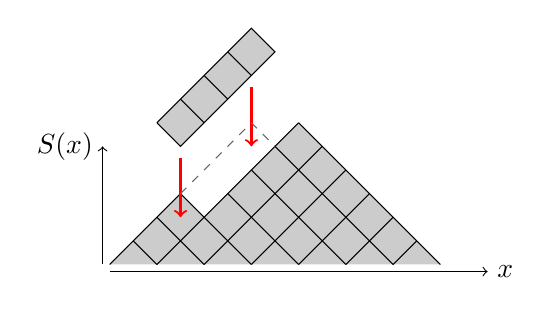
\begin{tikzpicture}[scale = .3]
\draw[->] (0, -.3) -- (16,-.3) node[right]{$x$};
\draw[->] (-.3,0) -- (-.3,5) node[left]{$S(x)$};
\fill[black!20] (0,0) -- (3,3) -- (4,2) -- (8,6) -- (14,0) ;
\draw (0,0) -- (3,3);
\draw (2,0) -- (8,6);
\draw (4,0) -- (9,5);
\draw (6,0) -- (10,4);
\draw (8,0) -- (11,3);
\draw (10,0) -- (12,2);
\draw (12,0) -- (13,1);
\draw (2,0) -- (1,1);
\draw (4,0) -- (2,2);
\draw (6,0) -- (3,3);
\draw (8,0) -- (5,3);
\draw (10,0) -- (6,4);
\draw (12,0) -- (7,5);
\draw (14,0) -- (8,6);

\draw[fill=black!20] (2,6) -- (3,5) -- (4,6) -- (5,7) -- (6,8) -- (7,9) --
					 (6,10) -- (3,7) -- (2,6);
\draw (4,6) -- (3,7);
\draw (5,7) -- (4,8);
\draw (6,8) -- (5,9);
%\draw (9,9) -- ()
\draw[thick, ->, red] (3,4.5) -- (3,2);
\draw[thick, ->, red] (6,7.5) -- (6,5);

\draw[dashed, black!60] (3,3) -- (6,6) -- (7,5);
\end{tikzpicture}
	\caption{\textbf{Near-maximal slope}. The single down step acts like a particle in the system. The 4 consecutive gates have the effect of moving the particle 3 sites to the right.}
	\label{fig:particle}
\end{figure}
Since gates can only act between a down step and an up step, these ``particles"\footnote{Define the particle as existing at site or cut?} follow a deterministic behavior and control the entropy growth in the circuit. 

Consider a series of consecutive gates with its first gate acting between sites $i$ and $i+1$ and its last gate between $j$ and $j+1$. Series of gates like this (called staircases) are discussed in section~\ref{sec:stairs}. If there are no down steps in this region, the gate has no effect. If there is a single down step between sites $i$ and $j$, inclusive, that step gets moved to site $j+1$. More down steps will interact with each other but at the present we are only considering configurations with isolated down steps. 

Now consider an operator with the last non-identity contribution at a site between $i$ and $j$, inclusive. With probability 1, the series of gates in the last paragraph move the end of the operator to site $j+1$. This should demonstrate that operator ends and down step ``particles" have the same dynamics. 

The speed of the end of the operator is $v_B$. It is not immediately clear how the speed of the particle, call it $v_p$, should be related. If, in time $t$ the particle moves $v_pt$ sites, it has increased the \dots

\emph{Finish this description. Does it really belong here though? If so, make sure to show that particles don't approach each other, but do repel each other if they're too close.}
\clearpage
\section{Dynamics in Asymmetric Circuits} \label{sec:stairs}

\subsection{Staircase Models} \label{sub:stairs}

An interesting generalization of the random architecture is to consider ``staircases," which each consist of a series of gates, acting at cuts $x$, $x+1$, $x+2$, in sequential order. This would be a staircase moving to the right, but they can also move to the left. If there are $n$ gates in a staircase it is called an $n$-stair. They are called staircases because compared to figure~\ref{fig:tetris} they look like steps, as in figure~\ref{fig:stairs}. 
\begin{figure}
	\centering
	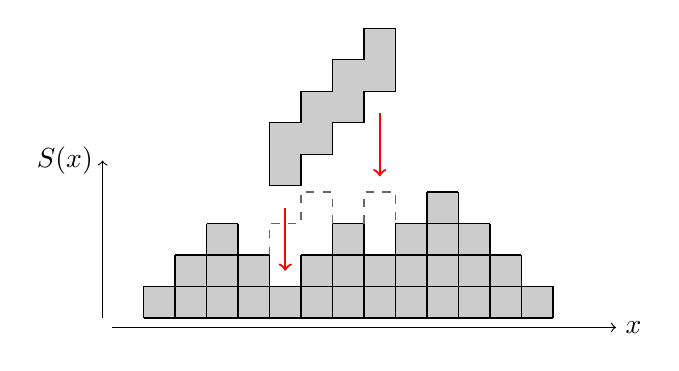
\begin{tikzpicture}[scale = .4]
\draw[->] (0, -.3) -- (16,-.3) node[right]{$x$};
\draw[->] (-.3,0) -- (-.3,5) node[left]{$S(x)$};
\fill[black!20] (1,0) -- (1,1) -- (2,1) -- (2,2) -- (3,2) -- (3,3) -- 
     			(4,3) -- (4,2) -- (5,2) -- (5,1) -- (6,1) -- (6,2) -- (7,2) -- (7,3) -- (8,3) -- (8,2) -- (9,2) -- (9,3) -- (10,3) -- (10,4) 
     			 -- (11,4) -- (11,3) -- (12,3) -- (12,2) -- (13,2) -- (13,1)  -- (14,1) -- (14,0);
     			 
\draw (1,0) -- (14,0);
\draw (1,1) -- (14,1);
\draw (2,2) -- (5,2);
\draw (6,2) -- (13,2);
\draw (3,3) -- (4,3);
\draw (7,3) -- (8,3);
\draw (9,3) -- (12,3);
\draw (10,4) -- (11,4);
\draw (1,0) -- (1,1);
\draw (2,0) -- (2,2);
\draw (3,0) -- (3,3);
\draw (4,0) -- (4,3);
\draw (5,0) -- (5,2);
\draw (6,0) -- (6,2);
\draw (7,0) -- (7,3);
\draw (8,0) -- (8,3);
\draw (9,0) -- (9,3);
\draw (10,0) -- (10,4);
\draw (11,0) -- (11,4);
\draw (12,0) -- (12,3);
\draw (13,0) -- (13,2);
\draw (14,0) -- (14,1);

\draw[fill=black!20] (5,5.2) -- (5,4.2) -- (6,4.2) -- (6,5.2) -- (7,5.2) --  
                     (7,6.2) --
					 (8,6.2) -- (8,7.2) -- (9,7.2) -- (9,8.2) -- (9,9.2) -- (8,9.2)
					 -- (8,8.2) -- (7,8.2) -- (7,7.2) -- (6,7.2) -- (6,6.2) -- (5,6.2)
					 -- (5,5.2);
\draw[thick, ->, red] (5.5,3.5) -- (5.5,1.5);
\draw[thick, ->, red] (8.5,6.5) -- (8.5,4.5);

\draw[dashed, black!60] (5,2) -- (5,3) -- (6,3) -- (6,4) -- (7,4) -- (7,3);
\draw[dashed, black!60] (8,3) -- (8,4) -- (9,4) -- (9,3);
\end{tikzpicture}
%\begin{tikzpicture}[scale = .3, cross/.style={path picture={ 
%		\draw[black]
%		(path picture bounding box.south east) -- (path picture bounding box.north west) (path picture bounding box.south west) -- (path picture bounding box.north east);
%}}]
%
%\draw[->] (0, -.3) -- (16,-.3) node[right]{$x$};
%\draw[->] (-.3,0) -- (-.3,5) node[left]{$S(x)$};
%\fill[black!20] (0,0) -- (3,3) -- (5,1) -- (7,3) -- (8,2) --
%(10,4) -- (14,0) ;
%\draw (0,0) -- (3,3);
%\draw (2,0) -- (4,2);
%\draw (4,0) -- (7,3);
%\draw (6,0) -- (10,4);
%\draw (8,0) -- (11,3);
%\draw (10,0) -- (12,2);
%\draw (12,0) -- (13,1);
%\draw (2,0) -- (1,1);
%\draw (4,0) -- (2,2);
%\draw (6,0) -- (3,3);
%\draw (8,0) -- (6,2);
%\draw (10,0) -- (7,3);
%\draw (12,0) -- (9,3);
%\draw (14,0) -- (10,4);
%\draw[dashed, black!60]  (5,3) -- (6,4);
%\draw[dashed, black!60]  (7,3) -- (6,4);
%\draw[dashed, black!60]  (6,2) -- (5,3);
%
%\draw[fill=black!20] (5,6) -- (6,5) -- (7,6) -- (6,7) -- (5,6);
%\draw[thick, ->, red] (6,4.5) -- (6,3);
%%\node [draw,circle,cross,minimum width=1](B) at (6,3.5){}; 
%\end{tikzpicture}

	\caption{\textbf{Staircase circuit architecture,} in which the gate at site $x$ is always followed by ones at sites $x+1, x+2$, making this a 3-stair. Note that not all gates are productive, only the ones that fall on sites that are local minima when they fall.}
	\label{fig:stairs}
\end{figure}
However, in the picture in which all sites are either up or down slopes, $n$-stair look like $n\times 1$ rectangles tilted $45^\circ$, as in figure~\ref{fig:diagstairs}.
\begin{figure}
	\centering
	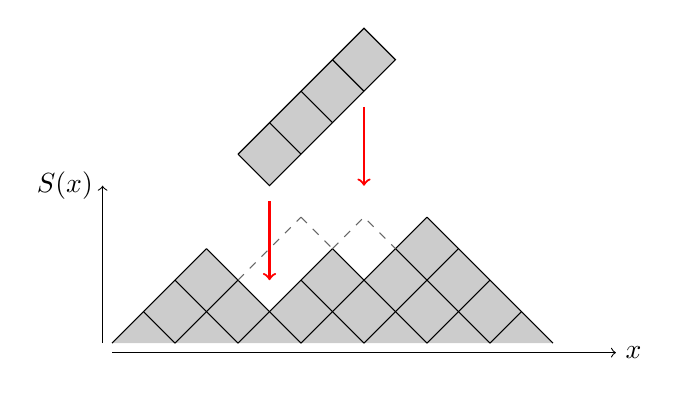
\begin{tikzpicture}[scale = .4]
\draw[->] (0, -.3) -- (16,-.3) node[right]{$x$};
\draw[->] (-.3,0) -- (-.3,5) node[left]{$S(x)$};
\fill[black!20] (0,0) -- (3,3) -- (5,1) -- (7,3) -- (8,2) --
				(10,4) -- (14,0) ;
\draw (0,0) -- (3,3);
\draw (2,0) -- (4,2);
\draw (4,0) -- (7,3);
\draw (6,0) -- (10,4);
\draw (8,0) -- (11,3);
\draw (10,0) -- (12,2);
\draw (12,0) -- (13,1);
\draw (2,0) -- (1,1);
\draw (4,0) -- (2,2);
\draw (6,0) -- (3,3);
\draw (8,0) -- (6,2);
\draw (10,0) -- (7,3);
\draw (12,0) -- (9,3);
\draw (14,0) -- (10,4);

\draw[fill=black!20] (4,6) -- (5,5) -- (6,6) -- (7,7) -- (8,8) -- (9,9) --
					 (8,10) -- (7,9) -- (6,8) -- (5,7) -- (4,6);
\draw (6,6) -- (5,7);
\draw (7,7) -- (6,8);
\draw (8,8) -- (7,9);
%\draw (9,9) -- ()
\draw[thick, ->, red] (5,4.5) -- (5,2);
\draw[thick, ->, red] (8,7.5) -- (8,5);

\draw[dashed, black!60] (4,2) -- (6,4);
\draw[dashed, black!60] (6,4) -- (7,3);
\draw[dashed, black!60] (7,3) -- (8,4) -- (9,3);
\end{tikzpicture}
%\begin{tikzpicture}[scale = .3, cross/.style={path picture={ 
%		\draw[black]
%		(path picture bounding box.south east) -- (path picture bounding box.north west) (path picture bounding box.south west) -- (path picture bounding box.north east);
%}}]
%
%\draw[->] (0, -.3) -- (16,-.3) node[right]{$x$};
%\draw[->] (-.3,0) -- (-.3,5) node[left]{$S(x)$};
%\fill[black!20] (0,0) -- (3,3) -- (5,1) -- (7,3) -- (8,2) --
%(10,4) -- (14,0) ;
%\draw (0,0) -- (3,3);
%\draw (2,0) -- (4,2);
%\draw (4,0) -- (7,3);
%\draw (6,0) -- (10,4);
%\draw (8,0) -- (11,3);
%\draw (10,0) -- (12,2);
%\draw (12,0) -- (13,1);
%\draw (2,0) -- (1,1);
%\draw (4,0) -- (2,2);
%\draw (6,0) -- (3,3);
%\draw (8,0) -- (6,2);
%\draw (10,0) -- (7,3);
%\draw (12,0) -- (9,3);
%\draw (14,0) -- (10,4);
%%\draw[dashed, black!60]  (5,3) -- (6,4);
%%\draw[dashed, black!60]  (7,3) -- (6,4);
%%\draw[dashed, black!60]  (6,2) -- (5,3);
%
%\draw[fill=black!20] (5,6) -- (6,5) -- (7,6) -- (6,7) -- (5,6);
%\draw[thick, ->, red] (6,4.5) -- (6,3);
%%\node [draw,circle,cross,minimum width=1](B) at (6,3.5){}; 
%\end{tikzpicture}

	\caption{\textbf{Another picture of the staircase architecture.} Note that this picture results in the same final state.}
	\label{fig:diagstairs}
\end{figure}

\subsection{Behavior Ignoring Correlations} \label{sub:anal}

Under certain approximations the entanglement entropy behaves analytically. One important approximation (described in section \ref{subsub:determ}) is that the Hilbert space at each site is large enough that almost all gates will in general maximally entangle the two sites on which they act. Other simplifying assumptions include ignoring correlations in ups and downs and ignoring second- and higher-order derivatives in $S(x,t)$. Combining these two assumptions, we arrive at uncorrelated entropy environments, which may be described only by their slope, $m$.

\subsubsection{Small Stairs} \label{subsub:smallstairs} 

The smallest stairs are 1-stairs, which are just individual gates. \emph{same as random circuit architecture, matches behavior there}

2-stairs consist of one gate acting at site $n$ and one at site $n+1$. The entropy production of these gates is affected by the slope between them and the two slopes on either side. There are 8 possible configurations of those three slopes, but only 4 result in entropy growth, as shown in table~\ref{tab:2stair}. Although there will be correlation built up by the 2-stair architecture, we can still make the assumption that there are no correlations. The average growth rate is then approximately 
\begin{align}
\pd{S}{t} = \Gamma\frac{1-m^2}{2}\frac{5+m}{4},
\end{align}
where $\Gamma$ is the rate of gates, so the rate of 2-stairs is $2\Gamma$.

\begin{table}
	\centering
	\begin{tabular}{ccc}
		Initial and Final 
		Configuration        & Probability         & Productivity\\
		$d\,u\,d\to u\,d\,d$ & $\frac{1-m^2}{4}\frac{1-m}{2}$ & 2\\
		$d\,u\,u\to u\,u\,d$ & $\frac{1-m^2}{4}\frac{1+m}{2}$ & 4\\
		$d\,d\,u\to d\,u\,d$ & $\frac{1-m^2}{4}\frac{1-m}{2}$ & 2\\
		$u\,d\,u\to u\,u\,d$ & $\frac{1-m^2}{4}\frac{1+m}{2}$ & 2
	\end{tabular}
	\caption{The four configurations that result in entropy growth for 2-stairs, their relative proportions assuming an uncorrelated entropy distribution, and the growth in entropy generated by a 2-stair falling on that configuration. The four configurations that do not result in entropy growth are $u\,u\,u, d\,d\,d, u\,d\,d,$ and $u\,u\,d$.}
	\label{tab:2stair}
\end{table}

\subsubsection{Larger Stairs}  \label{subsub:largestairs}

We can determine the growth rate for arbitrary length stairs through a recursive relationship. Consider a staircase made of $n$ gates. Its growth rate will be proportional to the gate rate normalized by the number of gates per stair, so we can write
\begin{align}
\pd{S}{t} = \frac{\Gamma}{n}R_n(m), \label{eqn:growthrate}
\end{align}
where $R_n(m)$ is the average entropy production of an $n$-stair. To find an equation for $R_n(m)$, note that the first $n-1$ gates have the same entropy production as the $(n-1)$-stair. Then the $n$th gate will produce another 2 units of entropy if the last step is up, but not if all $n+1$ steps are up. This is captured by the recursive formula
\begin{align}
R_n(m) = R_{n-1}(m)+2\frac{1+m}{2} - 2\left(\frac{1+m}{2}\right)^{n+1}. \label{eqn:raterecur}
\end{align}
Figure~\ref{fig:growthrates} contains a graph of some growth rates $\th{n}R_n(m)$ as a function of $m$.

\begin{figure}
	\centering
	\includegraphics[width=.5\textwidth]{analrates.png}
	\caption{Growth rates for 1-, 4-, 17-, and 100-stairs as a function of slope $m$. As stair length increases, the growth rate asymptotes to the function $\pd{S}{t} = m+1$.}
	\label{fig:growthrates}
\end{figure}

Note that with increasing stair length the growth rate asymptotes to the function $\pd{S}{t} = m+1$. There are two ways to reach this behavior. The first, which matches the order of the current reasoning, is to start with infinite spatial support and take the stair length $n\to\infty$. Alternatively, start with a finite spin chain with length $N$ and periodic boundary conditions, and set the stair length to $N$. Now a single gate acts on site $1,2,3\dots N$, before wrapping around to act at site 1 again. 

The maximal growth rate occurs when the slope is near-maximal, with only a single down step. This corresponds to a slope of $\frac{N-2}{N}$. Then with only a single local minimum in the entropy function, the local minimum moves one site to the right with each gate. Every gate that acts raises the entropy, resulting in an entropy gain of 2 per gate. Of course for a slope of 1, there is still no entropy generation.

If there are 2 down steps, for a slope of $\frac{N-4}{N}$, the entropy generation is almost the same. One local minimum still moves to the right with the leading edge of the staircase. However, once per staircase (once every $N$ gates), one down step is next to the other down step. This results in no entropy growth for that step, for an average entropy gain of $2\frac{N-1}{N}$. Further discussion of the dynamics with near-maximal slope appear in section~\ref{subsub:nearmax}.

This pattern continues as the slope decreases. With $\l$ down steps, the slope is $\frac{N-2\l}{N}$ and the average growth rate is $2\frac{N-\l}{N} = m+1$. At $m = -1$ there is no growth, as expected. At $m=0$, the growth rate is 1, the same as in the brickwork model. With no slope, the steps alternate between up and down, so that half of the gates in any stair are effective, explaining the connection to the brickwork model.

\subsection{Ergodicity and Stability}\footnote{The following section describes an attempt to calculate steady state correlations. I haven't been successful in doing this yet, but I wanted to write it up in case it proves useful.} \label{sub:erg}

A Markov process is one in which the future state depends only on the current state, not the past. Label the states $s_i$ and define $p_{i,t}$ as the probability that the system is in state $s_i$ at time $t$. When there is a constant probability $S_{ij}$ of transitioning from state $j$ to state $i$\footnote{Is this true of all Markov processes?} it is possible to write the transition matrix $S$ such that $p_{i,t+1}= S_{ij}p_{j,t}$. Since the product of the transition matrix and a probability vector gives the probabilities at the next time step, the transition matrix for $t$ time steps is just $S^t$. Under certain conditions\footnote{Figure these out.} the multi-step transition matrix approaches a constant matrix with all columns equal to the same vector $v^*$,
\begin{align}
\lim\limits_{t\to \infty}S^t = S^* = \begin{bmatrix}
\vdots & \vdots &  & \vdots\\
p^* & p^* & \cdots & p^*\\
\vdots & \vdots &  & \vdots\\
\end{bmatrix}.
\end{align}
Then the probability after a long time is the vector $p^*$ for any initial state.

The transition matrix can also be written as $S = 1+T$. The columns of $T$ must sum to 0 to preserve probabilities. From $S^*p^* = p^*,$ it must be true that $Tp^*=0$. This definition provides an easier route to finding $p^*$.

\subsubsection{Stable State in Random Architecture}  \label{subsub:randstate}

This analysis can be used to find the correlations present in the steady states of staircase architectures. Consider the 1-stair circuit, and enumerate 2-site (3-cut) states by the slope at the 2 sites: $s_1 = d\,d,\; s_2 = d\,u$, etc. Since at every time step there is an equal probability of a gate falling at any site, the transition matrix is the matrix product of single-cut transition matrices $P_{N} = \prod_NP_{1}\otimes$, where the single-cut transition matrix is 
\begin{align}
P_1 = \begin{bmatrix}
1-\frac{1+m}{2}\Gamma & 0      & \frac{1-m}{2}\Gamma & 0\\
\frac{1+m}{2}\Gamma & 1-\Gamma & 0                   & \frac{1-m}{2}\Gamma\\
0                   & \Gamma   & 1-\Gamma            & 0\\
0                   & 0        & \frac{1+m}{2}\Gamma & 1 - \frac{1-m}{2}\Gamma
\end{bmatrix}. \label{eqn:1sitetrans}
\end{align}
The $m$ dependence comes from the possibility of a gate acting on the left or right cut, which depends on the probability of the next slope being up or down.
The equilibrium state is
\begin{align}
v^* = \begin{pmatrix}
\frac{(1-m)^2}{4} \\ 
\frac{1+m}{2}\frac{1-m}{2} \\
\frac{1-m}{2}\frac{1+m}{2} \\
\frac{(1+m)^2}{4}
\end{pmatrix} = \begin{pmatrix}
\frac{1-m}{2} \\ \frac{1+m}{2}
\end{pmatrix} \otimes \begin{pmatrix}
\frac{1-m}{2} \\ \frac{1+m}{2}
\end{pmatrix},
\end{align}
which is uncorrelated, showing that the assumption of lack of correlation (used in equation~\ref{eqn:1sitetrans}) is consistent. Markov's theorem states that if all states are reachable from all other states\footnote{Probably introduce this earlier.} then the system is ergodic. An ergodic system contains only one equilibrium state, so the uncorrelated state is the unique equilibrium state.

\subsubsection{Stable States in Larger Staircases}  \label{subsub:stairstate}

Finding the stable state in the staircase models is more difficult. Since there are in fact correlations, a transition matrix built using the same method as in equation~\ref{eqn:1sitetrans} would be inexact. One possibility is to assume that the preceding and succeeding slopes are uncorrelated but to consider larger and larger subsystems (instead of the 2 slopes used previously).\footnote{I've made progress on this but haven't finished it.}

\subsection{Numerical Simulation} \label{sub:num}

To simulate the entropy growth in infinite spin chains with non-zero slope, we use finite chains with periodic boundary conditions, where one end of the chain is attached to the other with an offset. The spin chains are initialized with a highly correlated\footnote{A next step is to fix the initialization so that the states start uncorrelated.} entropy function with the given slope. Since larger gates will generate different correlation, growth rates are calculated for only the latter part of the simulation, ensuring that the entropy is in its equilibrium state.

\subsubsection{Measuring Growth Rates}  \label{subsub:growthrates}

Growth rates for stairs of various lengths are shown in figure~\ref{fig:compareRates}. As length increases, the growth rate follows the same pattern as predicted, increasing with the maximum moving right. 
\begin{figure}
	\centering
	\includegraphics[width=.5\textwidth]{compareRates.pdf}
	\caption{\textbf{Growth rates for different length stairs.} All growth rates were calculated using a 100-site spin chain with offset periodic boundary conditions. Rates were calculated from the application of 100,000 gates, averaged over the last 80\% of the gates in order to build up correlations.}
	\label{fig:compareRates}
\end{figure}

For 1-stairs (the random architecture), the measured growth rate is slightly larger than predicted, seen in figure~\ref{fig:1stairRates}.
\begin{figure}
	\centering
	\includegraphics[width=.5\textwidth]{1stairRates.pdf}
	\caption{\textbf{Measured and analytic growth rates} for the 1-stair architecture. Note that the measured rate is slightly higher. Since the assumption of un-correlation is exact for 1-stairs, this difference is assumed to be due to second order derivatives in the slope and finite length effects.}
	\label{fig:1stairRates}
\end{figure}
There are two main differences between the analytic and measured setups. For the analytic result, the chain is infinite and the entropy function is assumed to be linear and uncorrelated. Since the assumption of un-correlation is exact for 1-stairs, this difference is assumed to be due to second order derivatives in the slope and finite length effects.

Stairs of length greater than 1 do however generate correlations. Figure~\ref{fig:6stairRates} shows the growth rates for 6-stairs. 
\begin{figure}
	\centering
	\includegraphics[width=.5\textwidth]{6stairRates.pdf}
	\caption{\textbf{Measured and predicted growth rates} for the 6-stair architecture. The measured rate is now lower than predicted, implying that the correlations built up by the stairs act to lower their entropy production.}
	\label{fig:6stairRates}
\end{figure}
The notable difference in growth rate here is probably due to correlations created by the 6-stairs. Hopefully reasoning similar to that in section~\ref{sub:erg} will be able to predict the correlation so that its effect, at least to first order, can be calculated. This would allow a much closer approximation than that in figure~\ref{fig:6stairRates}

\subsubsection{Measuring Correlations}  \label{subsub:correlations}

The first step in understanding the difference between predicted and measured behavior is understanding the correlations introduced by the gates. Figure~\ref{fig:stairCorrel} shows the initial and final correlations for the 1- and 3-stair circuits. Both curves were created by averaging over the correlation in the second half of a 10,000 step run, averaged over 10 runs.
\begin{figure}
	\centering
	\includegraphics[width=.495\textwidth]{1stairCorrel}
	\includegraphics[width=.495\textwidth]{3stairCorrel}
	\caption{\textbf{Correlations created by 1- and 3-stair circuits.} The initial correlation curve shows that because of the initialization procedure the slope-0 state is perfectly anti-correlated. However, the correlation quickly equilibrates (see figure~\ref{fig:corrgrowth}). The 3-stair circuit reaches a more highly-correlated state than the 1-stair circuit.}
	\label{fig:stairCorrel}
\end{figure}
The 3-stair circuit indeed generates more correlation than the 1-stair circuit. 

Although the initial state is highly anticorrelated, the evolution of the circuit quickly removes this correlation, as shown in figure~\ref{fig:corrgrowth}.
\begin{figure}
	\centering
	\includegraphics[width=.5\textwidth]{corrgrowth.pdf}
	\caption{\textbf{Correlation Growth for 0 slope.} Although the state starts out artificially anticorrelated, the correlation equilibrates after 400-600 time steps.}
	\label{fig:corrgrowth}
\end{figure}
The correlation saturates after 400-600 time steps, meaning the correlation of the initial state is not as important as the overall slope. For 1-stairs the correlation should asymptote to 0, as it appears to do. An interesting next step would be a way to analytically predict the correlation built by each circuit.
\clearpage
\section{Conclusion} 

\subsection{Summary} \label{sub:sum}

In this thesis, we analyzed the operator and entanglement dynamics in two asymmetric systems, a system with a time-independent Hamiltonian and a quantum circuit. In the Hamiltonian system we used the OTOC to diagnose operator spreading and move toward finding a butterfly velocity. Studying operator spreading worked particularly well in the Hamiltonian system because the OTOC has a simple form for a spin chain with spin-$\half$ sites. In the circuit we used the entanglement dynamics to assess the entanglement and butterfly velocities. Entanglement dynamics were well suited to the circuit because of a simplification in the large $q$ limit, which allowed exact solvability after averaging over circuits. We provided an argument that $v_B$ as calculated using entanglement dynamics or operator spreading is the same in the circuit models.

We constructed the Hamiltonian out of local 3-site terms, with the individual terms asymmetric. We explored the dynamics of the Hamiltonian before explicitly calculating velocity dependent Lyapunov exponents $\lambda(v)$. Since $v_B$ is defined by $\lambda(v_B)=0$, we would expect $\lambda(v)$ to have a zero. However, due to the finite size of our system, the $\lambda(v)$ we measured did not have a zero. Despite this difficulty, $\lambda(v)$ was greater for right moving signals than for left moving signals for all velocities, implying that $v_{B+}>v_{B-}$ when these velocities are well defined.

The quantum circuits we considered are staircase circuits, where $n$ gates fall sequentially on consecutive sites. We used the large-$q$ limit to calculate entanglement growth rates of these circuits in the approximation that the staircases do not generate correlations in the entanglement $S(x)$. We then simulated these circuits to show that this approximation is incorrect, but does capture the gross shape of $S(x)$. 

We then measured the correlation of the simulated circuits, and showed that inserting this empirical correlation removes most of the error in growth rate. We also demonstrated that it is possible to analytically predict the correlation over different distances for different stair lengths, and that only a finite number of correlations affect the growth rate.

\subsection{Outlook}

For both systems, there are several improvements that can be made, both obvious and subtle. The simplest extension to the Hamiltonian model is to extend the chain to more sites. This is computationally difficult, but might reward the user with a close approximation to $v_B$. 

Other extensions include different Hamiltonians. For example, instead of having a multisite Hamiltonian that is a chain of 3-site Hamiltonians, one could build it out of 4-site Hamiltonians. Then each individual term could be the Hamiltonian whose unitary evolution is the 4-site swap. 

In a broader analysis, it could be worthwhile to search the space of possible Hamiltonians for the most asymmetric system. This thesis only studies the Hamiltonian that it does because the 3-site swap is an asymmetric unitary operator. However there could very well be a different 3-site Hamiltonian that, when chained together, gives a higher ratio of $v_{B+}/v_{B-}$. Searching the space of Hamiltonians would be difficult because the criterion for asymmetry is non-linear.

In the circuit system, the main improvement to be made is to better calculate the correlation, and to possibly come up with a closed form expression for $C_\l$ for $n$-stairs. This thesis indicates that if this were completed the growth rated could be calculated exactly, because the main discrepancies between calculated and measured growth rates were explained by the measured correlation. Furthermore, this thesis did not include detailed discussion of the  function $G(v)$, which encodes the shape of $S(x,t)$ as $t$ grows~\cite{Jonay17}.

Another topic discussed in Refs.~\cite{Nahum2017, Jonay18} is entanglement growth for higher dimensional systems. It might be interesting to introduce asymmetric, or direction-dependent, entanglement dynamics into these systems.
\clearpage
\printbibliography

\end{document}
